\section{Auswertung}
\label{sec:Auswertung}

\subsection{Temperaturmessung}
Der gemessene Offset am Anfang beträgt $U_{0,Anfang} = \SI{0,0075}{\milli\volt}$ und am Ende $U_{0,Ende} = \SI{0,0088}{\milli\volt}$
Der Mittelwert beträgt also $U_0 = \SI{}{\milli\volt}$.
$\delta U = U_i - U_0$ ist demnach die wahre Spannung.
Die Temperatur im Raum betrug in etwa $T_0 = \SI{297,6}{\kelvin}$
Im Folgenden sind die Messdaten für matt, schwarz, glänzend und weiß in jener Reihenfolge aufgeführt:
\\
(Tabelle 1-4)
\\
Im obrigen Diagramm wurden die Spannungen $\delta U_i$ gegen die Differenz $T^4 - T_0^4$ aufgetragen.
Es wird ein linearer Zusammenhang der Form
\begin{equation}
  f(x) = mx + b
\end{equation}
erwartet.
Für die Ausgleichsrechnung wurden folgende Formeln der linearen Regression verwendet:
Für die Steigung $m$ wurde die Formel
\begin{equation}
  m = \frac{\overline{(T^4 - T_0^4) \cdot \delta U_i}-\overline{T^4 - T_0^4}\cdot \overline{\delta U_i}}{\overline{(T^4 - T_0^4)²}-\overline{(T^4 - T_0^4)}^2}
\end{equation}
verwendet. Der Schnittpunkt mit der y-Achse wird durch
\begin{equation}
  b = \frac{\overline{(T^4 - T_0^4)²} \cdot \overline{\delta U_i}- \overline{T^4 - T_0^4} \cdot \overline{(T^4 - T_0^4)\cdot \delta U_i}}{\overline{(T^4 - T_0^4)²}-\overline{T^4 - T_0^4}²}
\end{equation}
beschrieben.
Für die Fehlerrechnung wurde jeweils die Formel für die kleinsten Quadrate verwendet, die für m
\begin{equation}
  \sigma_m = \sqrt{\frac{\sigma²}{N(\overline{(T^4 - T_0^4)²}-\overline{T^4 - T_0^4}²)}}
\end{equation}
und für b
\begin{equation}
  \sigma_m = \sqrt{\frac{\sigma² \cdot \overline{T^4 - T_0^4}}{N(\overline{(T^4 - T_0^4)²}-\overline{T^4 - T_0^4}²)}}
\end{equation}
lauten. Wobei 
Dauraus resultieren
\subsection{Abstandsmessung}


\begin{figure}
  \centering
  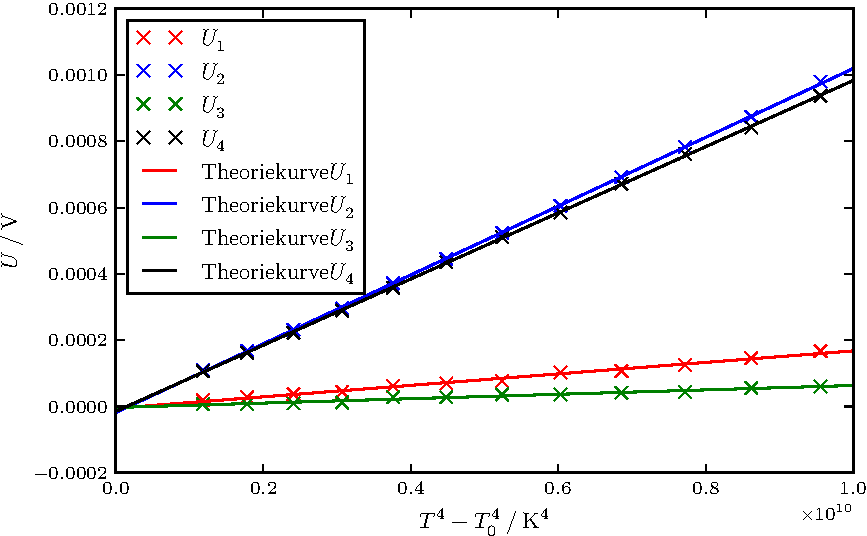
\includegraphics{plot.pdf}
  \caption{Plot.}
  \label{fig:plot}
\end{figure}
